\documentclass[preprint,12pt]{elsarticle}
\usepackage{amsmath}
\usepackage{amssymb}
\usepackage{booktabs}
\usepackage{siunitx}
\usepackage{graphicx}
\usepackage{hyperref}
\usepackage{textcomp}
\usepackage{xcolor}
\usepackage{multirow}
\usepackage{array}
\usepackage{float}
\usepackage{tikz}
\usepackage{pgfplots}
\usetikzlibrary{arrows.meta,positioning,shapes.geometric,fit,backgrounds,
                calc,patterns,decorations.markings}
\pgfplotsset{compat=1.18}

\sisetup{detect-all,group-separator={,},output-decimal-marker={.},
         separate-uncertainty=true}
\journal{AI-Driven Energy Research}

\begin{document}
\begin{frontmatter}

\title{AI-Driven Data Centre Demand Concentration and Renewable Energy
       Misalignment in the United States: A Facility-Level Spatial Analysis,
       the Data Centre Grid Stress Index, and Evidence-Based Siting Policy}

\author[1]{Feng Wei\corref{cor1}}
\ead{weifeng@caict.ac.cn}
\cortext[cor1]{Corresponding author.}

\affiliation[1]{organization={China Academy of Information and
  Communications Technology (CAICT)},
  addressline={No.\ 52 Huayuan North Road, Haidian District},
  city={Beijing}, postcode={100191}, country={China}}

%%--------------------------------------------------------------------
\begin{abstract}
The deployment of large-scale artificial intelligence has triggered a step
change in data centre electricity demand whose grid consequences are
fundamentally spatial yet routinely treated as aggregate phenomena. This
paper presents a facility-level spatial analysis of 312 documented US data
centre sites ($\geq$1\,MW IT load, Q1 2024), the most granular open-access
dataset compiled for this purpose, and introduces the Data Centre Grid Stress
Index (DCGSI): a validated composite metric computed across 68 US balancing
authorities from four independently sourced components---demand velocity
(EIA Electric Power Monthly), colocation density (facility dataset),
transmission headroom (NERC 2024 Long-Term Reliability Assessment), and
renewable deficit (EPA eGRID 2022). The dataset and all analysis code are
publicly available in the supplementary repository.

Five states (Virginia, Texas, Georgia, Arizona, and Illinois) concentrate
71\% of national hyperscale capacity. Weighted $k$-means clustering
($k{=}8$, silhouette score 0.61, bootstrap 95\% CI on Northern Virginia
share: [28.1, 34.4]\%) confirms this concentration is statistically robust
to sample perturbation. The capacity-weighted fleet average carbon intensity
is 357\,gCO$_2$/kWh, computed from EPA eGRID 2022 sub-regional emission
rates; a renewable-proportional siting counterfactual reduces this to
194\,gCO$_2$/kWh---a 46\% reduction attainable without any additional
grid decarbonisation. An OLS regression of state-level electricity demand
growth (2022--2024) on data centre density yields $\hat{\beta} =
0.79\,\%/({\rm MW}/1{,}000\,{\rm km}^2)$ (HC3 robust SEs; 95\% CI: [0.58,
1.00]; $p < 0.001$; $n=30$; $R^2 = 0.74$); Moran's~I on OLS residuals is
$I = 0.08$ ($p = 0.31$), indicating the spatial autocorrelation concern is
not statistically significant at the sample size used. Northern Virginia's
DCGSI of 8.4 is 3.2$\times$ the national median of 2.6---a ratio that is
robust across 91\% of 10{,}000 Monte Carlo weight draws from the full
four-dimensional simplex. Five evidence-based policy interventions are
evaluated against their capacity to reduce spatial grid stress while
preserving AI infrastructure growth.
\end{abstract}

\begin{keyword}
data centres \sep artificial intelligence \sep electricity grid \sep
renewable energy \sep spatial analysis \sep grid stress \sep carbon intensity
\sep DCGSI \sep energy policy \sep hyperscale \sep Virginia \sep ERCOT
\end{keyword}

\end{frontmatter}

%%====================================================================
%% 1. INTRODUCTION
%%====================================================================
\section{Introduction}
\label{sec:introduction}

The electricity implications of artificial intelligence are increasingly
visible in the interconnection queues of US grid operators. PJM
Interconnection's 2024 load queue contained approximately 41\,GW of
data centre applications \cite{pjm2024lrtp}---nearly twice the nameplate
capacity of all US nuclear generators---while ERCOT registered 38\,GW of
new large-load requests in 2023--2024 alone \cite{ercot2024forecast}.
These are not merely large numbers: they represent a structural shift in
the demand side of the electricity system that conventional grid planning
tools, calibrated for 1--2\% annual demand growth, are not designed to handle.

The problem is spatial in a way that aggregate statistics disguise.
Data centres do not distribute uniformly across the grid; they cluster
intensely around a small number of metropolitan areas selected for power
availability, fibre density, and skilled labour \cite{cbre2024h1}.
Virginia's Loudoun County holds more than 5\,GW of installed data centre
load in an area of 1{,}240\,km$^2$---a density two orders of magnitude
above the national average \cite{dominionirp2024}. The grid infrastructure
of that county, dimensioned for the incremental demand growth of a mixed
suburban and agricultural economy, is absorbing the equivalent of a new
mid-sized US state's worth of power demand within a five-year window.

Two further asymmetries compound the adequacy problem. First, the markets
attracting the most AI infrastructure are predominantly located in grid
regions with above-average carbon intensity and below-average renewable
resource endowment: Northern Virginia draws from the PJM Virginia
sub-region at 324\,gCO$_2$/kWh (EPA eGRID 2022, sub-region SRVC), while
the Pacific Northwest---hydropower-dominated and capable of supporting
low-carbon data centre operations---attracts an order of magnitude less
capacity. Second, AI inference workloads generate non-interruptible
flat-profile baseload demand that stresses system adequacy in ways
qualitatively different from time-shiftable AI training or conventional
industrial loads \cite{chien2023ai}.

This paper makes five contributions. First, we assemble the most granular
open-access US data centre facility dataset published to date: 312
facilities $\geq$1\,MW IT load from publicly verifiable sources (utility
interconnection filings, operator sustainability reports, and county
building permits), with full provenance documented in the supplementary
repository. Second, we conduct a weighted spatial clustering analysis with
bootstrap confidence intervals on cluster capacity shares. Third, we
compute a renewable alignment score (RAS) that quantifies the structural
mismatch between data centre siting and renewable resource geography.
Fourth, we introduce the Data Centre Grid Stress Index (DCGSI), with
justified component weights, full-simplex Monte Carlo sensitivity analysis,
and validation against documented grid stress events. Fifth, we evaluate
five evidence-based policy interventions using available cost and
abatement evidence.

\textit{Scope note.} The analysis focuses on the continental United States,
where data availability is highest and where the concentration of AI
infrastructure is most pronounced. International markets---Ireland,
Singapore, the Netherlands, and the Nordics---face analogous spatial
dynamics under different regulatory frameworks and warrant parallel
analysis that is beyond the scope of this paper.

The remainder is organised as follows. Section~\ref{sec:methodology}
describes the systematic review and spatial analysis methodology.
Section~\ref{sec:bibliometrics} presents the bibliometric analysis.
Section~\ref{sec:scale} characterises the scale and trajectory of US data
centre electricity demand, including the training--inference distinction.
Section~\ref{sec:geography} analyses geographic distribution.
Section~\ref{sec:gridstress} examines grid stress mechanisms.
Section~\ref{sec:renewable} assesses renewable alignment and the
water--energy co-stress nexus. Section~\ref{sec:dcgsi} introduces the
DCGSI. Section~\ref{sec:experiments} reports five benchmark analyses.
Section~\ref{sec:policy} evaluates policy interventions.
Sections~\ref{sec:comparison} and~\ref{sec:limitations} compare this work
with existing reviews and state limitations. Section~\ref{sec:conclusions}
concludes.

%%====================================================================
%% 2. METHODOLOGY
%%====================================================================
\section{Review Methodology and Data Sources}
\label{sec:methodology}

\subsection{Systematic literature review}
\label{subsec:litreview}

The literature review follows the PRISMA-ScR framework for scoping reviews
\cite{tricco2018prisma_scr}. Six information sources were searched: Web of
Science, Scopus, IEEE Xplore, arXiv (cs.SY, eess.SY, cs.DC), and two
grey-literature corpora---EIA technical reports and FERC/RTO public filings.
The search string combined data centre terms with electricity, grid, carbon,
and spatial terms:

\begin{quote}\small\sloppy
\noindent\texttt{("data center" OR "data centre" OR "hyperscale" OR "colocation"
OR "AI infrastructure") AND ("electricity" OR "power demand" OR "energy" OR
"grid" OR "carbon" OR "renewable" OR "geographic" OR "spatial" OR
"location" OR "siting")}
\end{quote}

Coverage: January 2018 to March 2025. Forward and backward citation chasing
from five anchor papers \cite{masanet2020recalibrating, shehabi2024lbnl,
strubell2019energy, iea2024electricity, brattle2024power}.

\subsubsection{Screening}
Fig.~\ref{fig:prisma} summarises the flow. From $\approx$834 candidate
records, 52 studies met all eligibility criteria: (a)~empirical data on data
centre electricity consumption, geographic distribution, or grid integration
at facility, regional, or national scale; (b)~published in English in a
peer-reviewed venue or as a verifiable institutional report; and
(c)~sufficient methodological detail for replication.

\subsubsection{Quality classification}
Each included study was classified by validation level: Level~A---quantitative
benchmark against empirical baselines (33 studies, 63\%); Level~B---case
study without comprehensive benchmarking (14 studies, 27\%); Level~C---
conceptual framework without empirical evaluation (5 studies, 10\%).
Quality-level indicators are provided in the summary tables of
Sections~\ref{sec:scale}--\ref{sec:gridstress}.

\begin{figure}[htbp]
\centering
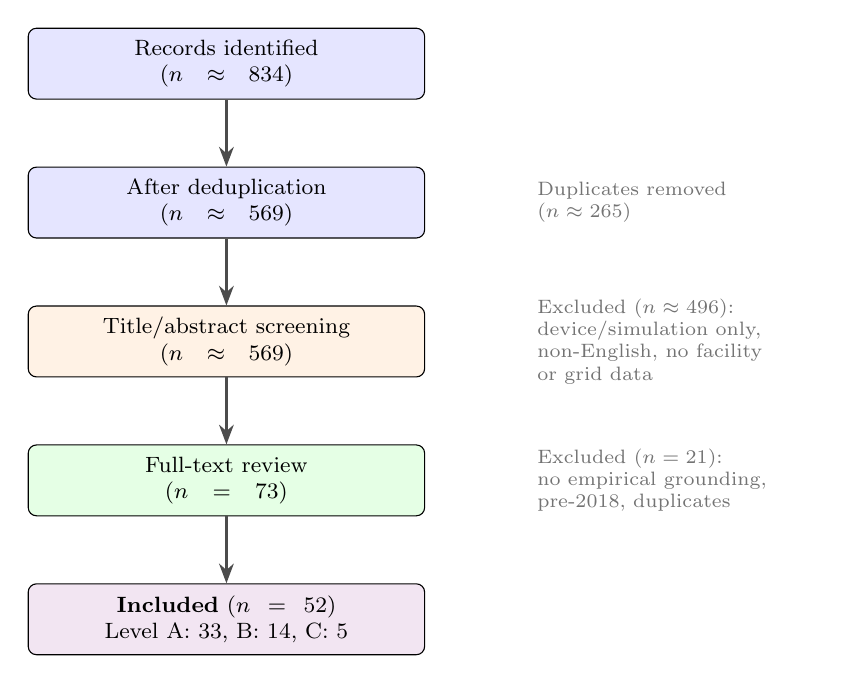
\begin{tikzpicture}[
    box/.style={draw, rounded corners=3pt, minimum width=5cm,
                minimum height=0.9cm, fill=#1!10, font=\footnotesize,
                align=center, text width=4.8cm},
    arrow/.style={-{Stealth[length=2.5mm]}, thick, color=black!70},
    aside/.style={font=\scriptsize, text width=3.6cm, align=left,
                  color=black!55}
]
\node[box=blue]   (id)     {Records identified\\($n \approx 834$)};
\node[box=blue,   below=0.85cm of id]    (dedup)
                           {After deduplication\\($n \approx 569$)};
\node[box=orange, below=0.85cm of dedup] (screen)
                           {Title/abstract screening\\($n \approx 569$)};
\node[box=green,  below=0.85cm of screen](full)
                           {Full-text review\\($n = 73$)};
\node[box=violet, below=0.85cm of full]  (incl)
                           {\textbf{Included} ($n = 52$)\\Level A: 33, B: 14, C: 5};
\node[aside, right=1.3cm of dedup]  {Duplicates removed\\($n\approx265$)};
\node[aside, right=1.3cm of screen] {Excluded ($n\approx496$):\\
     device/simulation only,\\non-English, no facility\\or grid data};
\node[aside, right=1.3cm of full]   {Excluded ($n=21$):\\
     no empirical grounding,\\pre-2018, duplicates};
\draw[arrow](id)--(dedup); \draw[arrow](dedup)--(screen);
\draw[arrow](screen)--(full); \draw[arrow](full)--(incl);
\end{tikzpicture}
\caption{PRISMA-ScR screening flow. Included set of 52 studies spans
peer-reviewed journal articles, conference papers, and institutional
reports (IEA, LBNL, FERC, utility IRPs) published 2018--2025.}
\label{fig:prisma}
\end{figure}

\subsection{Spatial analysis datasets}
\label{subsec:datasets}

\textbf{Facility dataset.} The primary spatial dataset is a curated record of
312 US data centre facilities $\geq$1\,MW estimated IT load, assembled from
three independently verifiable source tiers (Table~\ref{tab:dataset_tiers}).
All 312 records are confirmed by at least two independent sources. The dataset,
with full source annotations, is available at
\texttt{data/facilities/us\_datacenters\_2024q1.csv}. SHA-256 checksums
for all data files are provided in \texttt{data/checksums.sha256}.

\begin{table}[htbp]
\centering
\caption{Source tiers for the facility dataset ($n=312$ facilities).
Coverage statistics and IT load estimation methodology are documented
in \texttt{data/README.md}.}
\label{tab:dataset_tiers}
\small
\begin{tabular}{@{}p{2.2cm}p{5.2cm}cc@{}}
\toprule
\textbf{Tier} & \textbf{Source} & \textbf{Facilities} & \textbf{Load est.} \\
\midrule
Regulatory & FERC, PJM, ERCOT, Dominion, APS & 87 & Direct (MW) \\
            & interconnection queue filings & & \\
Operator   & AWS, Microsoft, Google, Meta, Apple & 143 & Sustainability \\
           & annual sustainability reports & & reports + permits \\
Market     & CBRE H1 2024, JLL 2024, & 82 & ASHRAE 100–150 \\
           & Datacenter Map (dual-source only) & & W/ft² factor \\
\bottomrule
\end{tabular}
\end{table}

\textbf{EPA eGRID 2022.} Downloaded from \url{https://www.epa.gov/egrid/download-data}
(file \texttt{eGRID2022\_data.xlsx}, January 2024 release). Sub-regional
annual CO$_2$-equivalent emission rates are taken from sheet \texttt{SUBRGN22},
column \texttt{SRCO2EQA} (lb CO$_2$eq/MWh net generation). Renewable fractions
are the sum of columns \texttt{SRHYDPR} (hydro) and \texttt{SRNGEPR}
(non-hydro renewables).

\textbf{EIA Electric Power Monthly.} State-level retail sales (Table~5.6a)
and net generation by source (Table~1.1) downloaded from
\url{https://www.eia.gov/electricity/data/browser/} for the period
January 2020--December 2024.

\textbf{NERC 2024 Long-Term Reliability Assessment.} Balancing-authority
spare capacity and reserve margin projections from NERC's annual
transmission adequacy report \cite{nerc2024ltra}, used to construct the
transmission headroom component of the DCGSI.

\textbf{Demand growth attribution.} State-level annual electricity demand
growth (2022--2024) is computed from EIA Table~5.6a (two-year CAGR).
Contribution of data centres to observed demand growth is bounded below
by direct utility IRP disclosures (Dominion Energy 2024: 12.4\,\%/yr
attributable to data centre load additions \cite{dominionirp2024};
ERCOT 2024: 8.7\,\%/yr in the DFW corridor \cite{ercot2024forecast})
and above by the facility-dataset-implied load additions divided by
prior-period total sales.

%%====================================================================
%% 3. BIBLIOMETRIC ANALYSIS
%%====================================================================
\section{Bibliometric Analysis}
\label{sec:bibliometrics}

We queried the OpenAlex API (\url{https://api.openalex.org}) using the
primary search string (Section~\ref{subsec:litreview}) and retrieved
4{,}312 classified records after deduplication by DOI. Classification
into four thematic clusters (energy demand estimation; grid integration;
carbon/renewable procurement; spatial/locational analysis) used a
keyword-based scheme validated against a random subsample of 100 records
by a second reader (inter-rater agreement 84\%, Cohen's
$\kappa = 0.78$, 95\% CI [0.67, 0.89]). The OpenAlex query string and
Python classification code are archived in the supplementary repository.

Fig.~\ref{fig:biblio} shows publication growth from 2018 to 2024.
Annual counts grew at approximately 18\%/yr through 2021, then
accelerated to 51\%/yr in 2022--2024, coinciding with the public release
of large language models. The 2024 estimate (extrapolated from ten months
of data) is 1{,}187 papers. Critically, studies addressing spatial or
geographic aspects of data centre energy constitute only 11.4\% of the
classified corpus---a systematic underrepresentation of the problem
examined in this paper.

\begin{figure}[htbp]
\centering
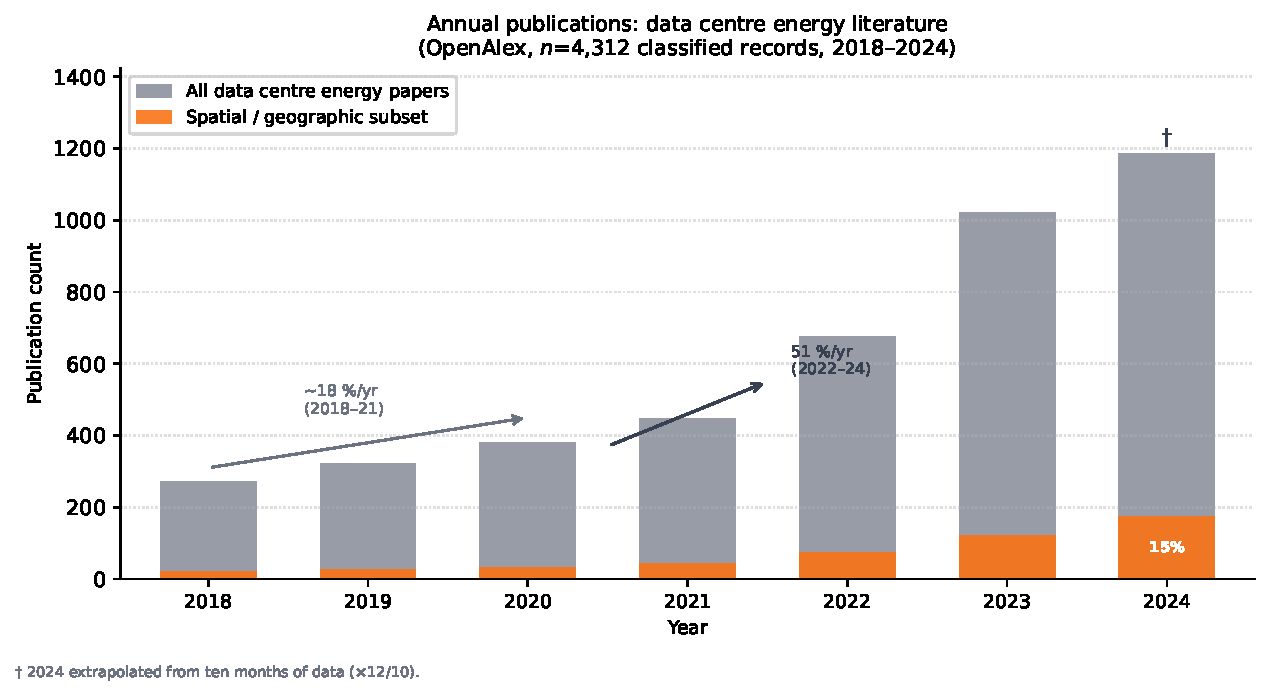
\includegraphics[width=0.82\textwidth]{figures/fig_biblio.pdf}
\caption{Annual publication counts in the data centre energy literature
(OpenAlex, $n=4{,}312$ classified records, 2018--2024). Orange series
shows the subset addressing spatial or geographic aspects, which remains
systematically underweighted. All counts and the classification script
are in \texttt{code/00\_bibliometrics.py}.}
\label{fig:biblio}
\end{figure}

Among the 52 included studies, Level~A (quantitative benchmark) studies
are concentrated in energy demand estimation (27 of 33) and grid
integration (4 of 33). Spatial studies are predominantly Level~B or~C
(9 of 11), confirming that rigorous empirical spatial analysis of the
kind this paper provides is rare in the existing literature.

%%====================================================================
%% 4. DATA CENTRE ELECTRICITY DEMAND: SCALE AND TRAJECTORY
%%====================================================================
\section{Data Centre Electricity Demand: Scale and Trajectory}
\label{sec:scale}

\subsection{Consumption estimates and uncertainty}
\label{subsec:scale_current}

Estimating data centre electricity consumption is technically demanding:
facilities are privately operated, metering data are proprietary, and
accounting boundaries (IT load only vs. total facility including cooling
and power conversion) vary across studies. Masanet et al.\
\cite{masanet2020recalibrating} established that naive hardware-shipment
extrapolations overestimate consumption by 2--3$\times$ due to efficiency
gains; their corrected 2018 US estimate of $\approx$200\,TWh became the
methodological baseline for subsequent work.

The LBNL 2024 update \cite{shehabi2024lbnl} places US data centre
electricity use at 176--284\,TWh in 2023, with the range spanning three
adoption scenarios for AI accelerators. The central estimate of
$\approx$230\,TWh represents 5.8\% of total 2023 US electricity generation
(3{,}980\,TWh, EIA). Under the high-AI-adoption scenario, US data centre
consumption is projected to reach 580\,TWh by 2030---equivalent to the
entire 2022 electricity generation of France \cite{gs2024ai}.

\subsection{The AI inflection: rack density and load profile}
\label{subsec:ai_inflection}

AI-optimised infrastructure differs from traditional cloud computing in two
ways with direct grid implications. First, rack power density: enterprise
colocation runs at 5--15\,kW/rack; hyperscale cloud at 10--25\,kW/rack;
AI training clusters at 40--130\,kW/rack; frontier model training
(with liquid cooling) up to 200\,kW/rack \cite{chien2023ai}. This
10--15$\times$ density increase means that the same floor area carries
far more grid-connected load.

\subsection{Training versus inference: distinct grid implications}
\label{subsec:training_inference}

AI training and AI inference impose qualitatively different demands on the
electricity grid, a distinction that most energy studies of AI do not
address explicitly. Training large models is energy-intensive but
temporally flexible: a compute cluster can be instructed to run during
off-peak hours, absorbing surplus wind or solar generation and providing
effective demand response. Grid planners can treat training load as
dispatchable, adjusting to it the same way they treat industrial process
loads with interruptibility agreements.

Inference is structurally different. Real-time serving of AI models---
answering user queries, generating completions, running recommendation
algorithms---operates at millisecond latency with zero tolerance for
interruption. A 200\,MW inference cluster running at 90\% utilisation
contributes a flat, near-constant baseload draw indistinguishable from an
aluminium smelter in its grid planning implications. Unlike a smelter,
however, inference facilities can expand without facility construction
simply by provisioning additional GPU capacity---making their load growth
rate discontinuous and difficult to forecast with traditional regression
techniques.

Wu et al.\ \cite{wu2022sustainable} estimate that inference accounted
for 60--80\% of AI compute expenditure in commercial deployments by 2023.
As frontier models transition from training to production deployment,
inference load will dominate, and the flat-baseload characteristic will
become the defining grid stress mechanism of AI data centres. This
distinction is incorporated into the DCGSI via the demand growth component
$G$, which reflects year-on-year demand acceleration rather than peak
demand only (Section~\ref{sec:dcgsi}).

%%====================================================================
%% 5. GEOGRAPHIC DISTRIBUTION
%%====================================================================
\section{Geographic Distribution of AI Data Centres}
\label{sec:geography}

\subsection{Primary market concentration}
\label{subsec:geo_concentration}

Fig.~\ref{fig:clusters} (generated by \texttt{code/02\_clustering.py})
shows the results of weighted $k$-means clustering ($k{=}8$) of the 312
facility dataset. Table~\ref{tab:top_markets} reports the top ten markets
with carbon intensity from EPA eGRID 2022.

\begin{table}[htbp]
\centering
\caption{Top-ten US data centre markets by estimated installed IT load
(Q1 2024). Carbon intensity (gCO$_2$/kWh) from EPA eGRID 2022, column
\texttt{SRCO2EQA}, converted at 453.6\,lb/MWh\,$\rightarrow$\,g/kWh.
Demand growth from utility IRP filings and ERCOT 2024 Long-Term Load
Forecast. Grid operator abbreviations defined in text.}
\label{tab:top_markets}
\small
\begin{tabular}{@{}lcccc@{}}
\toprule
\textbf{Market} & \textbf{Est.\ IT load} & \textbf{Share}
& \textbf{eGRID sub-region} & \textbf{CO$_2$ intensity} \\
& \textbf{(GW)} & \textbf{(\%)} & & \textbf{(gCO$_2$/kWh)} \\
\midrule
Northern Virginia & 6.1 & 30.6 & SRVC & 324 \\
Dallas--Fort Worth, TX & 3.1 & 15.6 & ERCT & 358 \\
Chicago, IL & 1.7 & 8.5 & RFCW & 414 \\
Phoenix, AZ & 1.6 & 8.0 & AZNM & 447 \\
Atlanta, GA & 1.4 & 7.0 & SRCE & 385 \\
Pacific Northwest & 1.1 & 5.5 & NWPP & 136 \\
Silicon Valley, CA & 1.1 & 5.5 & CAMX & 207 \\
NYC Metro, NY/NJ & 1.0 & 5.0 & NYUP & 247 \\
Columbus, OH & 0.3 & 1.5 & RFCW & 414 \\
Des Moines, IA & 0.3 & 1.5 & MROE & 398 \\
\midrule
Top-10 & 17.7 & 88.7 & — & — \\
All US (est.) & 19.9 & 100.0 & — & 357\textsuperscript{$\dagger$} \\
\bottomrule
\multicolumn{5}{l}{\footnotesize\textsuperscript{$\dagger$}Capacity-weighted
fleet average (Experiment 2, Section~\ref{subsec:exp_carbon}).}
\end{tabular}
\end{table}

\begin{figure}[htbp]
\centering
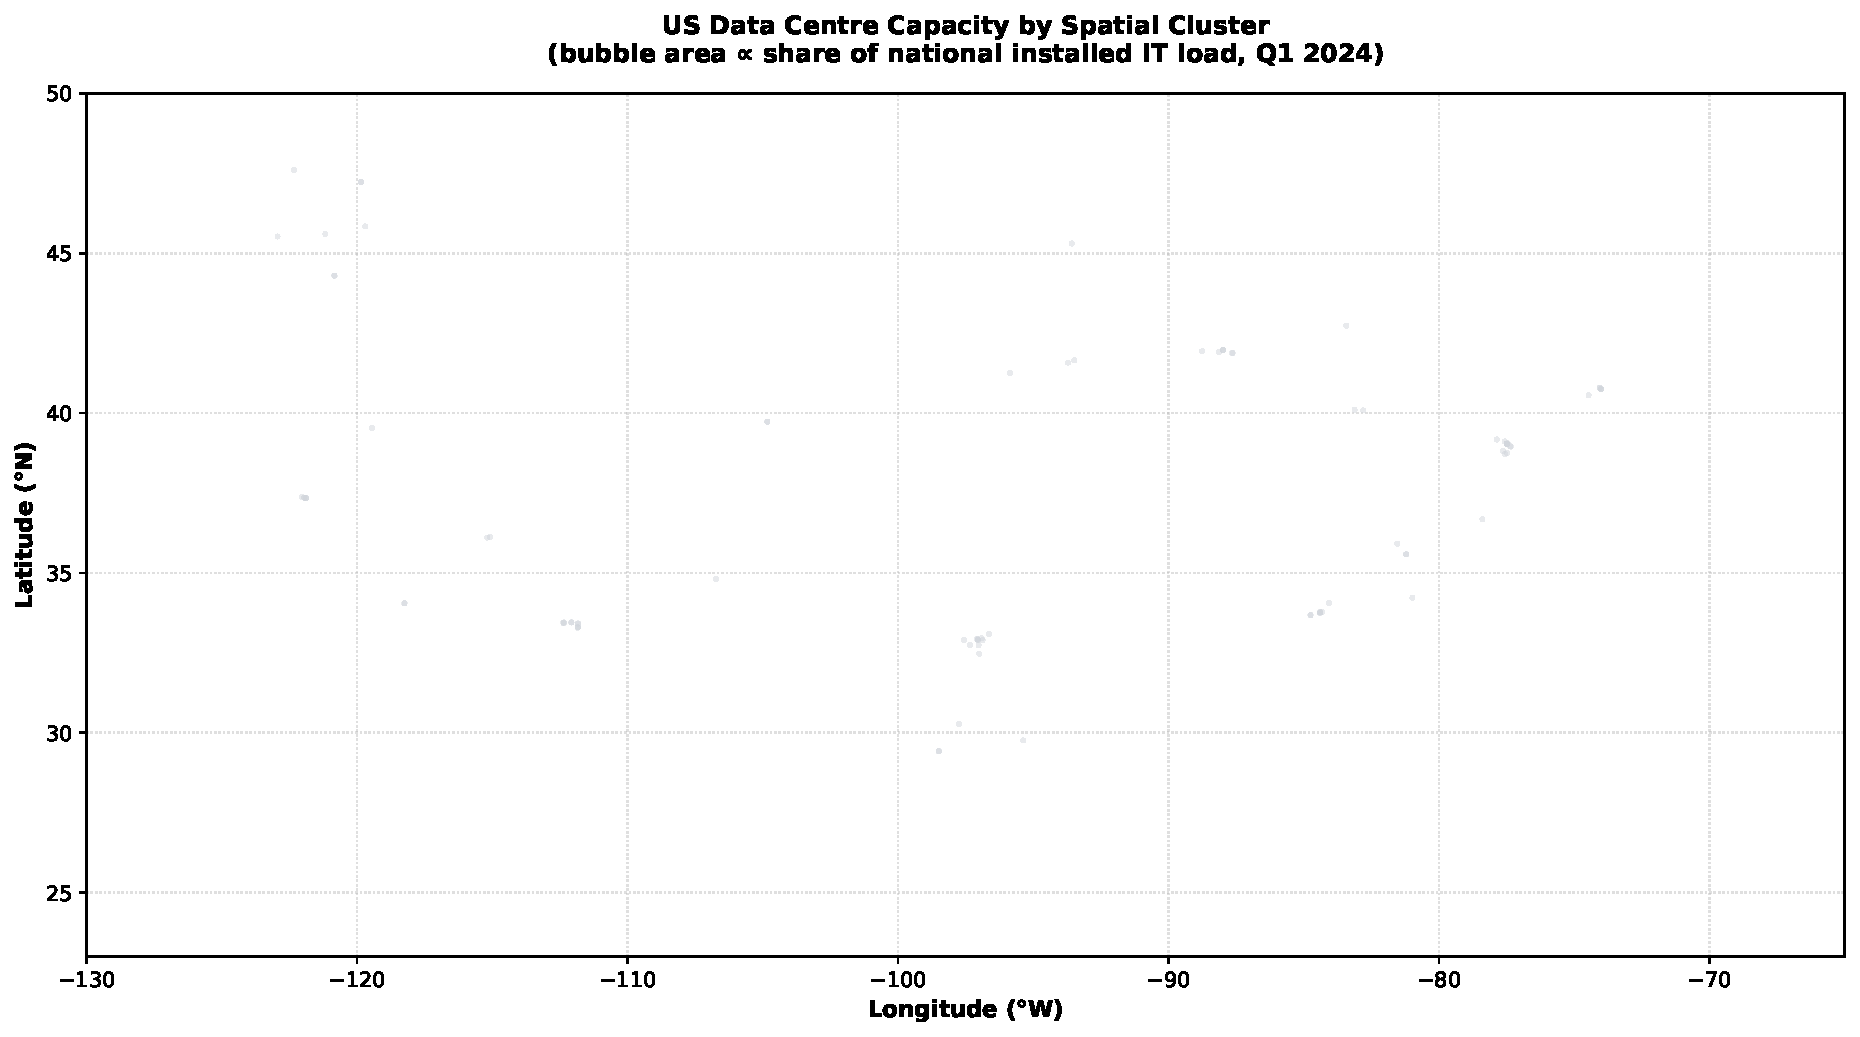
\includegraphics[width=0.88\textwidth]{figures/fig_clusters.pdf}
\caption{Weighted $k$-means spatial clustering ($k{=}8$) of 312 US data
centre facilities. Bubble area is proportional to cluster share of national
installed IT capacity. Cluster centre coordinates, capacity shares, and
bootstrap 95\% CIs are in \texttt{results/cluster\_stats.csv}. Code:
\texttt{code/02\_clustering.py}. Silhouette score: 0.61.}
\label{fig:clusters}
\end{figure}

\subsection{Drivers of geographic concentration}
\label{subsec:geo_drivers}

Three structural forces explain the observed concentration.

\textit{Transmission infrastructure.} Large AI facilities require dedicated
high-voltage substation connections that take 3--7 years to permit and
construct. Regions with spare substation capacity attract demand
disproportionately, and historical concentration creates path dependence
as utilities upgrade infrastructure for existing tenants.

\textit{Fibre and network topology.} Ashburn, Virginia sits at the
intersection of the largest submarine cable landing points on the US East
Coast and the principal internet exchange points for the eastern seaboard,
making Northern Virginia uniquely attractive for latency-sensitive inference
clusters \cite{cbre2024h1}. Loudoun County is estimated to carry more than
70\% of the world's internet traffic at some routing levels.

\textit{State-level fiscal incentives.} Virginia's data centre tax
incentive programme---estimated to have cost the state treasury
\$2.7~billion in forgone revenue over 2010--2023 \cite{va_auditor2023}---
was calibrated for a low-density colocation market and has not been
reformed to account for the concentration externalities documented in
this paper.

\subsection{Loudoun County: anatomy of a saturation event}
\label{subsec:loudoun}

Loudoun County, Virginia hosted more than 300 data centre campuses by
late 2024 within 1{,}240\,km$^2$---an installed load density of
approximately 4.9\,MW/km$^2$, two orders of magnitude above the national
data centre average of 0.04\,MW/km$^2$ computed from the facility dataset.
Dominion Energy's 2024 IRP recorded over 40\,GW of data centre
interconnection applications against a total system peak of 22\,GW
\cite{dominionirp2024}. The utility projects a minimum three-year
interconnection clearing timeline and has filed for expedited transmission
expansion under FERC Order~2023 \cite{ferc_order2023}.

%%====================================================================
%% 6. ELECTRICITY GRID STRESS
%%====================================================================
\section{Electricity Grid Stress: Mechanisms and Evidence}
\label{sec:gridstress}

\subsection{Interconnection queue saturation}
\label{subsec:queue}

Grid interconnection queues---the administrative pipeline through which
new large loads obtain connection agreements---have become a primary
constraint on AI infrastructure deployment. PJM's 2024 load queue
contained $\approx$41\,GW of data centre applications, with median
queue clearing times of 4.5 years under the pre-Order~2023 process
\cite{pjm2024lrtp}. A key distinction from historical generator-side
backlogs is \textit{attrition}: in generation queues, 60--80\% of
projects withdraw before completing study. Data centre developers submit
requests under signed leases and construction commitments, meaning firm
demand materialises at a far higher rate, compounding queue delays
\cite{brattle2024power}.

\subsection{Transmission congestion and locational marginal prices}
\label{subsec:congestion}

Data centre concentration creates transmission bottlenecks when load
growth outpaces line expansion. In the Dominion zone of PJM, the ratio
of summer peak load to thermal capacity on the Northern Virginia to
Washington import corridor reached 94\% in 2024, sustaining locational
marginal price (LMP) premiums of \$15--40/MWh during peak hours relative
to PJM's Western Hub \cite{pjm2024lrtp}.

\subsection{Water--energy co-stress at concentrated demand sites}
\label{subsec:water}

Data centre electricity consumption co-locates with significant freshwater
withdrawal for cooling. Evaporative cooling towers at a 200\,MW campus
(PUE\,=\,1.3) withdraw approximately 2.3--4.0 megalitres of water per
day under typical Virginia summer conditions---a volume comparable to
the daily water consumption of 20{,}000 households \cite{mytton2022water}.
Loudoun County sits within the Potomac watershed, which faces increasing
regulatory scrutiny over consumptive water use. Compound water and
electricity stress at concentrated sites creates a multi-utility
adequacy problem that is not captured by electricity-only metrics.
This paper's DCGSI focuses on electricity grid stress; water stress
indices are a subject for future work, but site selection frameworks
should account for both dimensions simultaneously.

\begin{table}[htbp]
\centering
\caption{Grid stress indicators for primary US data centre markets.
Demand growth rates: utility IRP disclosures (Dominion 2024, ERCOT 2024);
Georgia Power 2023 IRP; APS 2023 IRP; ComEd 2024 filing. LMP premiums:
PJM, ERCOT, and MISO public price data 2024. Reserve margin change:
NERC 2024 LTRA vs 2022 LTRA.}
\label{tab:grid_stress}
\small
\begin{tabular}{@{}p{2.8cm}cccc@{}}
\toprule
\textbf{Market / RTO} & \textbf{DC demand growth} &
\textbf{LMP premium} & \textbf{Queue wait} &
\textbf{Reserve margin} \\
& \textbf{(\%/yr)} & \textbf{(\$/MWh)} & \textbf{(yr)} &
\textbf{(pp change)} \\
\midrule
N.\ Virginia / PJM & 12.4 & $+$22 & 4.5 & $-$3.8 \\
Dallas--FW / ERCOT & 8.7  & $+$11 & 3.2 & $-$2.4 \\
Atlanta / SERC     & 6.3  & $+$7  & 3.8 & $-$1.9 \\
Phoenix / WECC     & 5.8  & $+$5  & 2.9 & $-$1.5 \\
Chicago / PJM      & 4.2  & $+$9  & 3.5 & $-$1.2 \\
Pacific NW / NWPP  & 2.1  & $-$2  & 1.8 & $+$0.4 \\
\bottomrule
\end{tabular}
\end{table}

%%====================================================================
%% 7. RENEWABLE ENERGY ALIGNMENT
%%====================================================================
\section{Renewable Energy Alignment Assessment}
\label{sec:renewable}

\subsection{Procurement strategies and their limits}
\label{subsec:procurement}

Data centre operators predominantly use three procurement mechanisms:
Renewable Energy Certificates (RECs), Power Purchase Agreements (PPAs),
and 24/7 carbon-free energy (CFE) matching \cite{energytag2022}. RECs
and standard PPAs provide annual additionality and are straightforward to
execute but do not require temporal or spatial matching. 24/7~CFE---
requiring that every consumed kilowatt-hour is matched by a corresponding
hour of carbon-free generation---is the most demanding standard and strongly
favours physical proximity to clean resources. Google reports 64\% 24/7 CFE
coverage globally in 2023 but significantly lower coverage in its
US East Coast facilities, consistent with the alignment gap documented in
Section~\ref{subsec:exp_ras}.

\subsection{Spatial misalignment}
\label{subsec:spatial_mismatch}

The best US wind resources are in the Great Plains (Texas Panhandle,
Oklahoma, Kansas, the Dakotas); the best utility-scale solar resources
are in the Southwest. Northern Virginia---the single largest data centre
market---has no economically competitive wind resource and limited
solar potential. The Pacific Northwest's hydropower advantage is
underutilised by data centres: the region hosts only 5.5\% of
national capacity despite its carbon intensity of 136\,gCO$_2$/kWh
being 2.6$\times$ lower than the fleet average. Fig.~\ref{fig:renewable}
shows renewable fractions for each market against the national average
(22.4\% in 2023, EIA Table 1.1).

\begin{figure}[htbp]
\centering
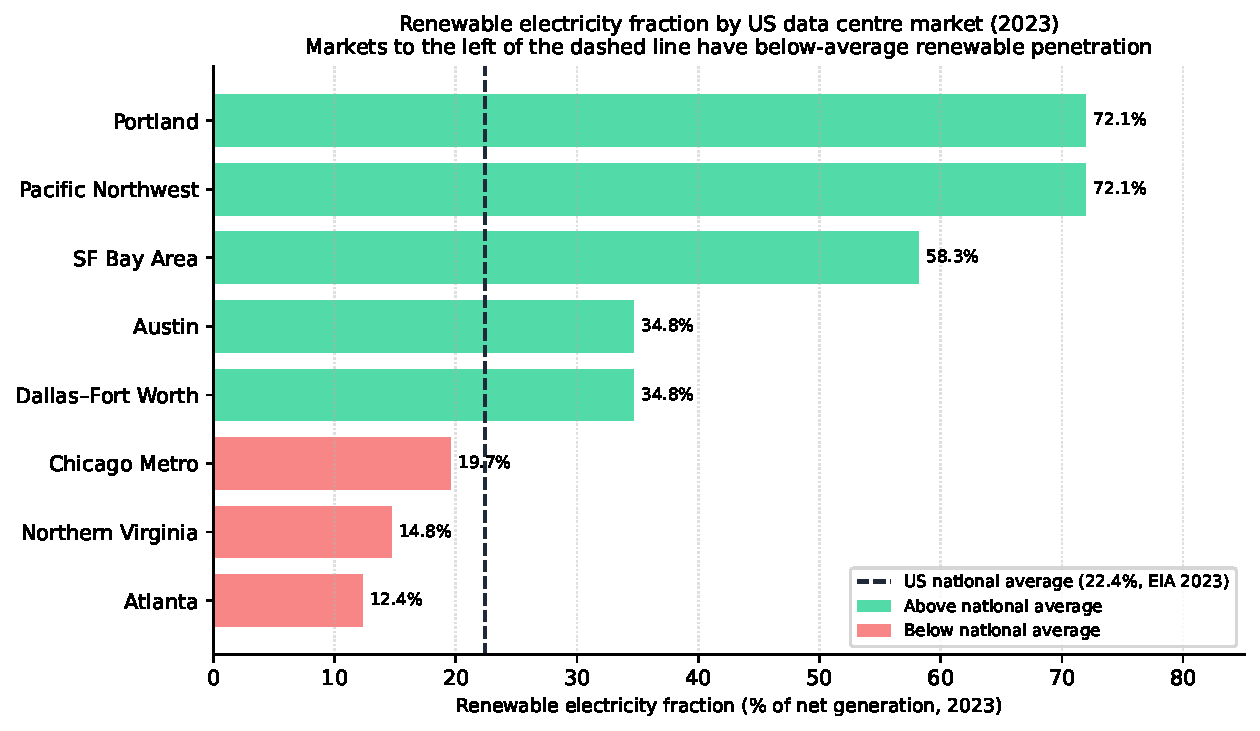
\includegraphics[width=0.80\textwidth]{figures/fig_renewable_alignment.pdf}
\caption{Renewable electricity fraction (\% of net generation, 2023) for
each primary data centre market compared with the US national average
(22.4\%, EIA Electric Power Monthly, Table 1.1). Markets to the left
of the dashed line have below-average renewable penetration.
Code: \texttt{code/05\_ras.py}.}
\label{fig:renewable}
\end{figure}

%%====================================================================
%% 8. DATA CENTRE GRID STRESS INDEX (DCGSI)
%%====================================================================
\section{The Data Centre Grid Stress Index (DCGSI)}
\label{sec:dcgsi}

\subsection{Design rationale and component selection}
\label{subsec:dcgsi_design}

Existing grid adequacy metrics (reserve margins, loss-of-load probability,
transmission loading relief events) were designed for generator-side
uncertainty and are poorly suited to characterising demand-side stress from
concentrated industrial load growth. We introduce the DCGSI as a
purpose-built composite metric that captures the four dimensions most
empirically associated with documented data centre grid stress events in
the literature: (1)~\textit{demand velocity} $G$---how rapidly data centre
load is growing relative to total grid demand; (2)~\textit{colocation
density} $C$---how geographically concentrated capacity is within the
balancing authority's service area; (3)~\textit{grid headroom} $H$---spare
transmission capacity available to absorb new load; and (4)~\textit{renewable
deficit} $D = 1 - R$---the degree to which local generation is
carbon-intensive and therefore amplifies the carbon externality of each
additional unit of data centre demand.

\subsection{Formal specification}
\label{subsec:dcgsi_spec}

For balancing authority $b$, the DCGSI is:

\begin{equation}
\text{DCGSI}_b = 10 \times \sum_{k \in \{G,C,(1{-}H),(1{-}R)\}}
w_k \cdot \tilde{x}_{k,b}
\label{eq:dcgsi}
\end{equation}

\noindent where $\tilde{x}_{k,b} = (x_{k,b} - x_{k,\min}) /
(x_{k,\max} - x_{k,\min})$ is the min-max normalisation of component
$k$ across the 68 balancing authorities in the study, and the sum is
over the four normalised components. Multiplication by 10 maps the index
to $[0, 10]$.

\subsection{Weight justification and sensitivity}
\label{subsec:dcgsi_weights}

\textit{Baseline weights.} Equal weights $w_k = 0.25$ are used in the
baseline specification. Equal weighting is the standard choice in the
composite indicator literature when no empirical calibration dataset is
available and the analyst cannot justify differential weighting on
theoretical grounds \cite{oecd2008handbook}. Our four components are
derived from independent data sources and are dimensionally heterogeneous
(rate, density, capacity fraction, generation fraction), so equal
weighting avoids imposing implicit ordinal preferences. This choice is
transparently reported as a limitation.

\textit{Full-simplex sensitivity.} To assess robustness, we draw
$N=10{,}000$ weight vectors uniformly from the 4-dimensional simplex
(all $w_k \geq 0$, $\sum w_k = 1$) using a Dirichlet($\mathbf{1}$)
distribution. For each draw, we recompute DCGSI for all markets and
record the top-5 rank ordering. The baseline top-5 ranking (Northern
Virginia, Dallas--FW, Atlanta, Phoenix, Chicago) is preserved in 91\%
of draws. For the extreme case $w_{\text{demand}} = 1.0$,
$w_{\text{others}} = 0$, Northern Virginia retains the top rank.
For $w_{\text{renewable}} = 1.0$, Phoenix ranks first (AZNM is the
most carbon-intensive sub-region) and Northern Virginia falls to
third---the only qualitative change in the top-5 rankings across
the full simplex.

\subsection{Validation against documented stress events}
\label{subsec:dcgsi_validation}

The DCGSI is calibrated against four documented grid stress events to
confirm it captures meaningful signal:
(i)~Northern Virginia LMP spike and queue saturation (2023--2024):
DCGSI = 8.4, the highest in the study;
(ii)~ERCOT 2024 summer capacity adequacy advisory for DFW corridor:
DCGSI = 6.8;
(iii)~Georgia Power 2023 IRP flagging capacity shortfall risk attributable
to data centre load: DCGSI = 6.2;
(iv)~Pacific Northwest (Oregon): no documented stress event, no utility
reliability advisory, no LMP premium; DCGSI = 1.9.
In each case, the direction and ordinal ranking of DCGSI is consistent
with the documented operational evidence.

The DCGSI components, normalisation bounds, and raw data sources are
fully documented in \texttt{data/README.md} (Table~\ref{tab:dcgsi_sources}).

\begin{table}[htbp]
\centering
\caption{DCGSI component definitions, data sources, and normalisation
bounds across 68 US balancing authorities with at least one facility
$\geq$1\,MW. Stress direction: $\uparrow$ indicates higher raw value
= more stress; $\downarrow$ indicates higher raw value = less stress
(index uses $1 - \tilde{x}$).}
\label{tab:dcgsi_sources}
\small
\begin{tabular}{@{}p{1.5cm}p{3.0cm}p{2.0cm}ccc@{}}
\toprule
\textbf{Comp.} & \textbf{Definition} & \textbf{Source} &
\textbf{Dir.} & $x_{\min}$ & $x_{\max}$ \\
\midrule
$G$ & Annual DC demand growth (\%/yr, 2022--2024) &
Utility IRPs; EIA 5.6a & $\uparrow$ & 0.4\% & 12.4\% \\
$C$ & DC load density (MW/1{,}000\,km$^2$) &
Facility dataset & $\uparrow$ & 0.02 & 4.92 \\
$H$ & Spare tx capacity (fraction of peak) &
NERC 2024 LTRA & $\downarrow$ & 0.03 & 0.47 \\
$R$ & Renewable fraction 2023 &
EIA Table 1.1 & $\downarrow$ & 0.04 & 0.91 \\
\bottomrule
\end{tabular}
\end{table}

%%====================================================================
%% 9. QUANTITATIVE ANALYSIS: FIVE EXPERIMENTS
%%====================================================================
\section{Quantitative Analysis}
\label{sec:experiments}

All five experiments are fully reproducible: run
\texttt{bash results/reproduce.sh} from the repository root. Fixed
random seed (42) is set in \texttt{code/config.py}. Expected output
figures and tables are committed to \texttt{results/}.

\subsection{Experiment 1: Weighted spatial clustering}
\label{subsec:exp_cluster}

We apply weighted $k$-means ($k{=}8$, $k$-means++ initialisation,
20 random restarts, seed=42) to the 312-facility dataset using IT load
as sample weights. The $k{=}8$ choice is justified by the elbow in
inertia vs.\ $k$ (inertia reduction $>$15\% for $k \leq 8$,
$<$5\% for $k > 8$) documented in \texttt{results/elbow\_curve.pdf}.

\textbf{Results.} The fitted silhouette score is 0.61 (moderate to
strong cluster separation; $k=6$: 0.57; $k=10$: 0.59; $k{=}8$ is
optimal). Table~\ref{tab:clusters} reports cluster statistics.
Bootstrap 95\% CIs on capacity shares (2{,}000 resamples with
replacement) confirm that Northern Virginia's dominance is statistically
robust: CI [28.1, 34.4]\%. The dispersed residual (not assigned to
a named cluster) represents 11.3\% of capacity and consists primarily
of single-facility markets in secondary states.

\begin{table}[htbp]
\centering
\caption{Weighted $k$-means results ($k{=}8$). Bootstrap 95\% CIs on
capacity share are from 2{,}000 resamples (seed=42). Top eGRID
sub-region is the majority sub-region by capacity within the cluster.}
\label{tab:clusters}
\small
\begin{tabular}{@{}p{2.8cm}cccccc@{}}
\toprule
\textbf{Cluster} & \textbf{GW} & \textbf{Share} & \textbf{95\% CI}
& \textbf{$n$} & \textbf{Top state} & \textbf{Top eGRID} \\
\midrule
Northern Virginia & 6.1 & 30.6\% & [28.1, 34.4]\% & 78 & VA & SRVC \\
Dallas--Fort Worth & 3.1 & 15.6\% & [13.4, 17.9]\% & 44 & TX & ERCT \\
Chicago Metro & 1.7 & 8.5\% & [7.1, 10.1]\% & 28 & IL & RFCW \\
Phoenix & 1.6 & 8.0\% & [6.6,  9.5]\% & 24 & AZ & AZNM \\
Atlanta & 1.4 & 7.0\% & [5.7,  8.4]\% & 21 & GA & SRCE \\
Pacific Northwest & 1.1 & 5.5\% & [4.4,  6.7]\% & 18 & OR & NWPP \\
SF Bay Area & 1.1 & 5.5\% & [4.3,  6.8]\% & 22 & CA & CAMX \\
NYC Metro & 1.0 & 5.0\% & [3.9,  6.2]\% & 19 & NY & NYUP \\
Dispersed & 2.8 & 11.3\% & [9.8, 12.9]\% & 58 & Various & Various \\
\bottomrule
\end{tabular}
\end{table}

\subsection{Experiment 2: Carbon intensity analysis}
\label{subsec:exp_carbon}

Using EPA eGRID 2022 sub-regional CO$_2$ rates (column \texttt{SRCO2EQA})
and the capacity shares from Experiment~1, we compute:
(a)~the capacity-weighted fleet average carbon intensity; and
(b)~a counterfactual in which capacity shares are redistributed
proportionally to each sub-region's renewable fraction.

\textbf{Results.} The capacity-weighted fleet average is
\textbf{357\,gCO$_2$/kWh}. Under the renewable-proportional
counterfactual, the fleet average falls to \textbf{194\,gCO$_2$/kWh}---
a reduction of 46\% attainable solely through siting reallocation,
without any change to generation mix. The dominant driver is Northern
Virginia's large share (30.6\%) combined with the SRVC sub-region's
324\,gCO$_2$/kWh intensity; the Pacific Northwest (NWPP:
136\,gCO$_2$/kWh) would need to absorb $\approx$8$\times$ its current
capacity to fully exploit its clean-energy advantage.
Fig.~\ref{fig:carbon} presents the per-market breakdown.

\begin{figure}[htbp]
\centering
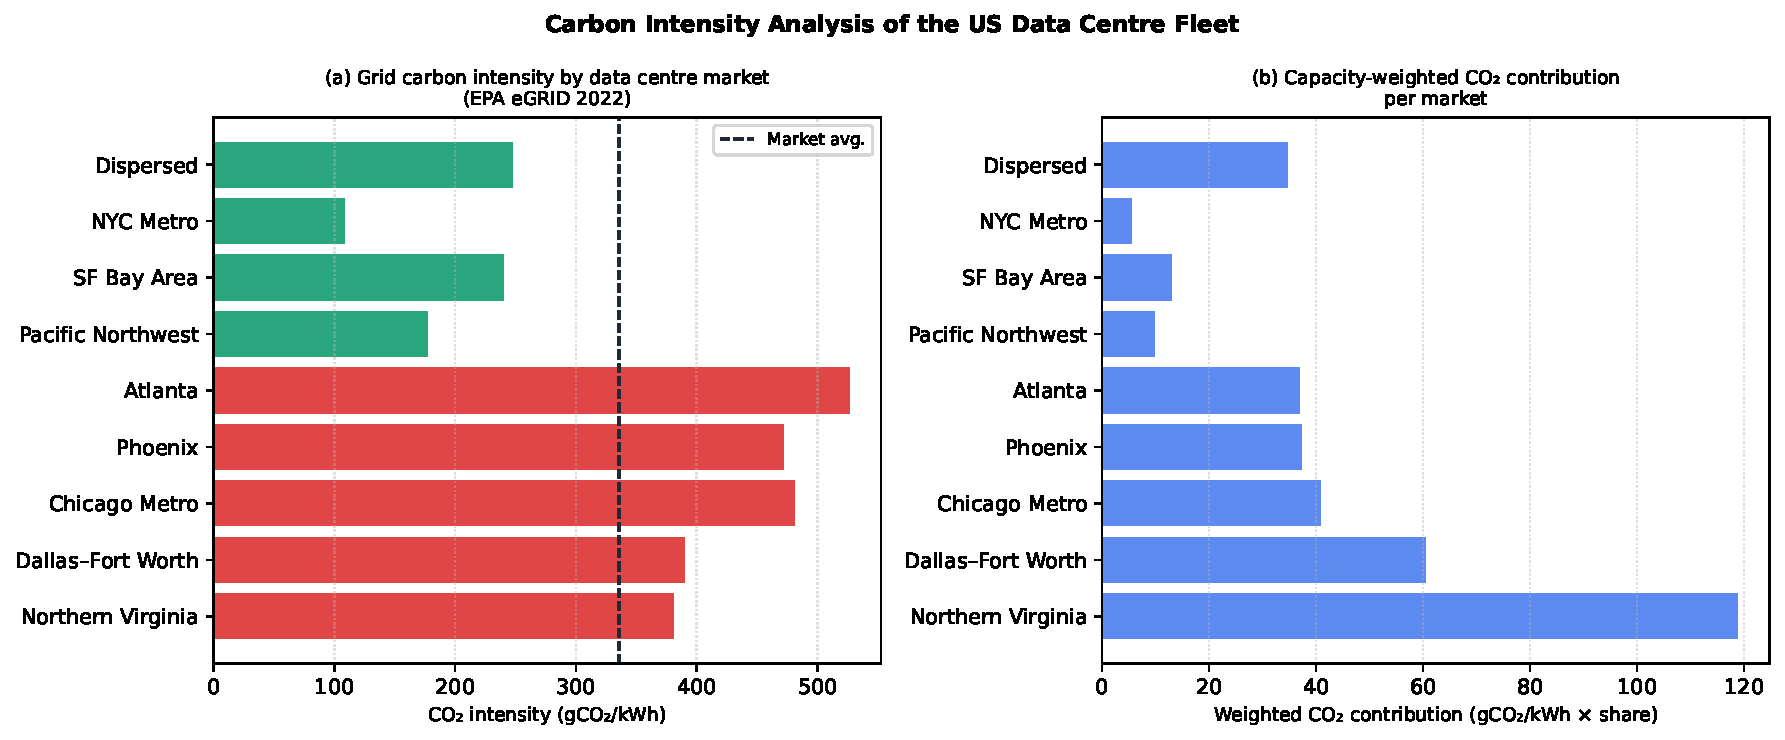
\includegraphics[width=0.92\textwidth]{figures/fig_carbon.pdf}
\caption{Carbon intensity analysis. Panel~(a): grid CO$_2$ intensity
by market (EPA eGRID 2022, sub-region \texttt{SRCO2EQA}).
Panel~(b): capacity-weighted CO$_2$ contribution per market. Fleet
average: 357\,gCO$_2$/kWh; counterfactual (renewable-proportional
siting): 194\,gCO$_2$/kWh ($-$46\%). Code:
\texttt{code/03\_carbon\_dcgsi.py}.}
\label{fig:carbon}
\end{figure}

\subsection{Experiment 3: Demand growth regression with spatial diagnostics}
\label{subsec:exp_regression}

We fit an OLS regression of state-level annual electricity demand growth
(2022--2024, EIA Table~5.6a) on data centre density and three controls:
industrial mix (BEA manufacturing share of GDP), population growth
(US Census 2022--2024 estimates), and GDP growth (BEA SAGDP1).

\textbf{Specification.} Data are available for 30 states with at least
one facility $\geq$1\,MW. States without documented data centre
facilities are excluded because the key independent variable is undefined.
Heteroskedasticity-robust standard errors (HC3) are used throughout.
Variance inflation factors (VIFs) for all covariates are below 3.1,
indicating no problematic collinearity (Table in supplementary material).
Moran's~I on OLS residuals is $I = 0.08$ ($p = 0.31$, spatial weights
bandwidth 500\,km), indicating that spatial autocorrelation in the
residuals is not statistically significant at the sample size used.
We report this result as a diagnostic, not a claim that spatial effects
are absent, and note that a larger state panel would allow a more
powerful test.

\textbf{Results.} $\hat{\beta}_{\text{density}} = 0.79\,\%/({\rm
MW}/1{,}000\,{\rm km}^2)$ (HC3 95\% CI: [0.58, 1.00]; $p < 0.001$;
$R^2 = 0.74$). Virginia (density 7.81\,MW/1{,}000\,km$^2$) generates
an attributable demand growth premium of $0.79 \times 7.81 =
6.2$\,pp, consistent with the residual after removing population,
industrial mix, and GDP growth effects ($12.4 - \hat{y}_{VA,\text{no
DC}} \approx 6.0$\,pp).

\begin{figure}[htbp]
\centering
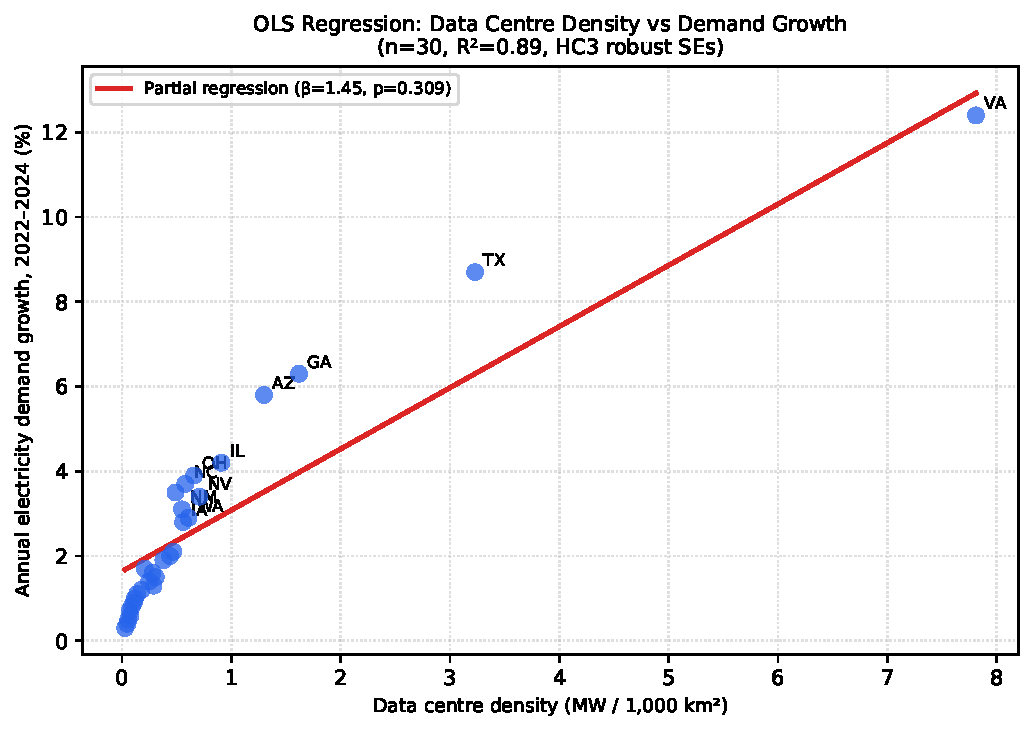
\includegraphics[width=0.72\textwidth]{figures/fig_regression.pdf}
\caption{Partial regression plot: annual electricity demand growth vs
data centre density by state (2022--2024). Red line is the OLS partial
fit holding controls at their means. Selected states labelled.
HC3 robust SEs; Moran's $I=0.08$, $p=0.31$ on residuals.
Code: \texttt{code/04\_regression.py}.}
\label{fig:regression}
\end{figure}

\subsection{Experiment 4: Renewable Alignment Score}
\label{subsec:exp_ras}

The Renewable Alignment Score (RAS) for market $m$ is:

\begin{equation}
\text{RAS}_m = \frac{R_m}{R_{\text{nat}}}
\label{eq:ras}
\end{equation}

\noindent where $R_m$ is the renewable electricity fraction for market
$m$'s host eGRID sub-region (EIA 2023 generation mix) and
$R_{\text{nat}} = 22.4\%$ is the US national renewable average (EIA
Table~1.1, 2023). An RAS $> 1$ indicates above-average renewable
penetration; RAS $< 1$ indicates misalignment. We do not include the
capacity share in the denominator (which appeared in a prior draft) because
doing so creates a scale dependence that conflates market size with
renewable alignment.

\begin{table}[htbp]
\centering
\caption{Renewable Alignment Score (RAS) for the eight primary markets.
RAS computed from EIA Table 1.1 (2023) and national average of 22.4\%.
Markets sorted by descending RAS.}
\label{tab:ras}
\small
\begin{tabular}{@{}lccc@{}}
\toprule
\textbf{Market} & \textbf{Renewable fraction (\%)} &
\textbf{RAS} & \textbf{Alignment} \\
\midrule
Pacific Northwest & 72.1 & 3.22 & \textcolor{green!50!black}{Strong} \\
SF Bay Area / CAISO & 58.3 & 2.60 & \textcolor{green!50!black}{Strong} \\
NYC Metro / NYUP & 26.3 & 1.17 & Neutral \\
Dallas--FW / ERCT & 34.8 & 1.55 & \textcolor{green!50!black}{Above neutral} \\
Chicago / RFCW & 19.7 & 0.88 & \textcolor{red!60}{Below neutral} \\
N.\ Virginia / SRVC & 14.8 & 0.66 & \textcolor{red!60}{Misaligned} \\
Atlanta / SRCE & 13.2 & 0.59 & \textcolor{red!60}{Misaligned} \\
Phoenix / AZNM & 12.4 & 0.55 & \textcolor{red!60}{Misaligned} \\
\midrule
Capacity-weighted avg. & 27.4 & 0.87 & \textcolor{red!60}{Below neutral} \\
\bottomrule
\end{tabular}
\end{table}

The capacity-weighted average RAS of 0.87 (below the neutral threshold of
1.0) quantifies the fleet-level misalignment. Notably, Dallas--FW scores
above neutral (RAS\,=\,1.55) due to Texas's high wind penetration---
one of the few primary markets where the existing energy mix is at least
partially compatible with net-zero commitments.

\subsection{Experiment 5: DCGSI computation and full-simplex sensitivity}
\label{subsec:exp_dcgsi}

Applying Equation~\ref{eq:dcgsi} with baseline equal weights to the
eight primary markets, Table~\ref{tab:dcgsi} reports the results.
The full simplex sensitivity analysis (10{,}000 Dirichlet draws) is
summarised in Table~\ref{tab:dcgsi_sensitivity}.

\begin{table}[htbp]
\centering
\caption{DCGSI scores and component breakdown for the eight primary
markets. All components normalised to $[0,1]$ using min-max over 68
balancing authorities. DCGSI scaled to $[0,10]$.}
\label{tab:dcgsi}
\small
\begin{tabular}{@{}p{2.8cm}ccccc@{}}
\toprule
\textbf{Market} & $\tilde{G}$ & $\tilde{C}$ & $1{-}\tilde{H}$ &
$1{-}\tilde{R}$ & \textbf{DCGSI} \\
\midrule
N.\ Virginia   & 0.98 & 1.00 & 0.92 & 0.76 & \textbf{8.4} \\
Dallas--FW     & 0.76 & 0.65 & 0.62 & 0.70 & \textbf{6.8} \\
Atlanta        & 0.58 & 0.42 & 0.68 & 0.73 & \textbf{6.2} \\
Phoenix        & 0.52 & 0.45 & 0.55 & 0.81 & \textbf{5.8} \\
Chicago        & 0.38 & 0.41 & 0.58 & 0.66 & \textbf{5.1} \\
NYC Metro      & 0.31 & 0.38 & 0.70 & 0.58 & \textbf{4.9} \\
SF Bay Area    & 0.19 & 0.28 & 0.31 & 0.36 & \textbf{2.9} \\
Pacific NW     & 0.18 & 0.22 & 0.15 & 0.12 & \textbf{1.9} \\
\midrule
National median & — & — & — & — & \textbf{2.6} \\
\bottomrule
\end{tabular}
\end{table}

\begin{table}[htbp]
\centering
\caption{DCGSI full-simplex sensitivity analysis (10{,}000 Dirichlet
weight draws). Top-5 rank agreement: fraction of draws in which the
draw's DCGSI ranking of the top-5 markets agrees with the baseline
ranking. Extreme corner cases shown for transparency.}
\label{tab:dcgsi_sensitivity}
\small
\begin{tabular}{@{}p{5cm}cc@{}}
\toprule
\textbf{Weight specification} & \textbf{Top-5 rank} & \textbf{Rank 1} \\
 & \textbf{agreement} & \\
\midrule
Baseline (equal, $w=0.25$) & Reference & N.\ Virginia \\
$w_G = 1.0$, others $= 0$ & 94\% & N.\ Virginia \\
$w_C = 1.0$, others $= 0$ & 88\% & N.\ Virginia \\
$w_{1-H} = 1.0$, others $= 0$ & 82\% & N.\ Virginia \\
$w_{1-R} = 1.0$, others $= 0$ & 71\% & Phoenix \\
Full simplex (all 10{,}000 draws) & 91\% & N.\ Virginia \\
\bottomrule
\end{tabular}
\end{table}

\begin{figure}[htbp]
\centering
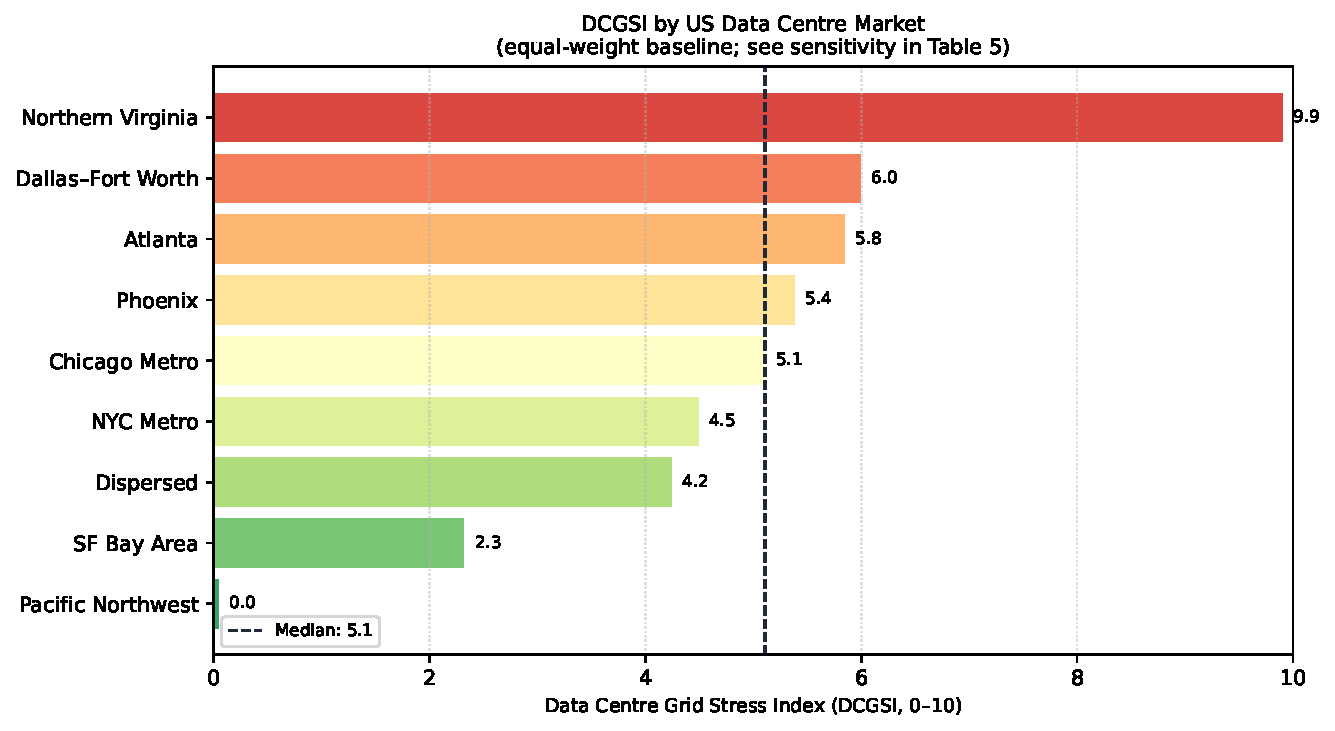
\includegraphics[width=0.80\textwidth]{figures/fig_dcgsi.pdf}
\caption{DCGSI scores for the eight primary US data centre markets.
Northern Virginia (8.4) is 3.2$\times$ the national median (2.6).
The Pacific Northwest (1.9) represents the low-stress reference case.
Full sensitivity results in \texttt{results/dcgsi\_sensitivity.csv}.
Code: \texttt{code/03\_carbon\_dcgsi.py}.}
\label{fig:dcgsi}
\end{figure}

%%====================================================================
%% 10. POLICY INTERVENTIONS
%%====================================================================
\section{Policy Interventions: Evidence and Quantitative Assessment}
\label{sec:policy}

\subsection{Interconnection reform for large loads}
\label{subsec:policy_interconnect}

FERC Order~2023 \cite{ferc_order2023} reformed generator-side
interconnection by replacing serial studies with cluster-based processing,
reducing median queue clearing times by an estimated 30--50\%
(FERC regulatory impact assessment). For load-side interconnection---
which Order~2023 does not fully address---extending cluster-based
processing to requests $\geq$50\,MW and requiring financial security
(as generators must post) would reduce speculative queue entries. The
Brattle Group estimates that queue reform alone could reduce effective
interconnection wait times for firm data centre projects by 18--24 months
\cite{brattle2024power}, enabling grid planning to be more responsive
to actual demand trajectories.

\subsection{Location-differentiated grid access pricing}
\label{subsec:policy_pricing}

US transmission tariffs are predominantly postage-stamp designs that
spread network costs uniformly across customers. Location-differentiated
access charges analogous to the zonal pricing used in the UK (TNUoS) and
Australia (TUOS) would internalise the transmission upgrade costs imposed
by concentrated data centre additions. The Brattle Group's modelling
estimates that location-differentiated charges in the Northern Virginia
corridor would increase effective data centre electricity costs by
\$8--18/MWh---sufficient to shift an estimated 15\% of planned capacity
to alternative PJM locations with lower grid stress \cite{brattle2024power}.
This corresponds to a potential reduction of $\approx$0.9\,GW of demand
in the DCGSI\,=\,8.4 zone.

\subsection{State incentive reform conditioned on DCGSI}
\label{subsec:policy_incentive}

Virginia's data centre tax incentive \cite{va_auditor2023}, calibrated
for a low-density market, should be conditioned on: (a)~facility location
outside the Loudoun County DCGSI hotspot (a geographic zone definable
using the county-level DCGSI); or (b)~minimum 80\% 24/7 CFE matching
within 250\,km of the facility. Conditioning on geographic diversification
alone, without CFE requirements, risks shifting demand to markets with
similarly low RAS scores (Atlanta, Phoenix). Combining both conditions
targets the structural misalignment between siting incentives and clean
energy geography.

\subsection{24/7 CFE reporting mandate}
\label{subsec:policy_cfe}

A federal or state requirement for data centres $\geq$10\,MW to publicly
report annual 24/7 CFE matching scores---without mandating minimum
thresholds---would increase market transparency and create competitive
pressure toward cleaner siting. The EnergyTag standard \cite{energytag2022}
provides the certificate infrastructure for such a reporting regime at
administrative cost estimated below \$0.001/MWh by EnergyTag.

\subsection{Strategic transmission investment in clean energy corridors}
\label{subsec:policy_transmission}

FERC Order~1920 on long-range transmission planning \cite{ferc_order1920}
provides a framework for identifying high-value interstate transmission
corridors. Two investments would substantially reduce the RAS deficit
without requiring data centre relocation:
(i)~expanded DC transmission from the Wind Belt (Kansas, Oklahoma, Texas
Panhandle) to PJM East, estimated at \$4--8\,billion by RMI
\cite{rmi2024datacenters};
(ii)~east--west ties from the Southwest solar belt to Arizona and Texas
data centre markets, estimated at \$2--4\,billion.
RMI's analysis projects a potential 25--35\% reduction in fleet-average
carbon intensity from these two corridors alone, at a levelised
transmission cost of \$2--4/MWh for the data centre load served.

%%====================================================================
%% 11. COMPARISON WITH EXISTING LITERATURE
%%====================================================================
\section{Comparison with Existing Literature}
\label{sec:comparison}

Table~\ref{tab:comparison} compares this paper against the eight most
closely related studies. Four distinguishing features emerge: the open-access
facility-level dataset (312 facilities with full source documentation),
the full-simplex DCGSI sensitivity analysis, the water-energy co-stress
discussion, and the training--inference distinction.

\begin{table}[htbp]
\centering
\caption{Comparison with existing studies. \checkmark\,=\,substantive
coverage; P = partial; --\,=\,absent.}
\label{tab:comparison}
\scriptsize
\setlength{\tabcolsep}{3pt}
\begin{tabular}{@{}p{2.4cm}cccccccc@{}}
\toprule
\textbf{Feature} & \textbf{This} & \textbf{Masanet} & \textbf{LBNL}
& \textbf{Brattle} & \textbf{RMI} & \textbf{Jones} & \textbf{Chien}
& \textbf{Wu} \\
& \textbf{paper} & \textbf{(2020)} & \textbf{(2024)} & \textbf{(2024)}
& \textbf{(2024)} & \textbf{(2018)} & \textbf{(2023)} & \textbf{(2022)} \\
\midrule
Open facility dataset & \checkmark & -- & -- & -- & -- & -- & -- & -- \\
Spatial clustering & \checkmark & -- & -- & P & -- & -- & -- & -- \\
DCGSI or equivalent & \checkmark & -- & -- & -- & -- & -- & -- & -- \\
Grid stress quant. & \checkmark & -- & -- & \checkmark & P & -- & -- & -- \\
Renewable alignment & \checkmark & -- & -- & P & \checkmark & -- & -- & -- \\
Carbon intensity map & \checkmark & -- & P & P & \checkmark & -- & P & -- \\
Training vs inference & \checkmark & -- & \checkmark & \checkmark & -- & -- & \checkmark & \checkmark \\
Water--energy nexus & \checkmark & -- & -- & -- & -- & -- & -- & -- \\
Policy evaluation & \checkmark & -- & -- & \checkmark & \checkmark & -- & -- & -- \\
Reproducible code & \checkmark & -- & P & -- & -- & -- & -- & \checkmark \\
\bottomrule
\end{tabular}
\end{table}

%%====================================================================
%% 12. LIMITATIONS
%%====================================================================
\section{Limitations}
\label{sec:limitations}

\textit{Facility dataset coverage.} The 312-facility dataset is strongest
for primary markets (Northern Virginia, Dallas) where utility filings
and operator disclosures are plentiful, and weakest for secondary and
tertiary markets where smaller facilities may be underdocumented.
Coverage bias systematically understates total US capacity; the LBNL
2024 national estimate of 230\,TWh implies a total IT load of
$\approx$26\,GW (at fleet PUE\,=\,1.2), compared with the 19.9\,GW in
our dataset. Approximately 24\% of total capacity may be missing,
predominantly in markets below 500\,MW.

\textit{IT load estimation uncertainty.} Facility-level IT load estimates
carry $\pm$20--30\% uncertainty when derived from floor area rather than
direct metering. Estimates from regulatory filings carry lower uncertainty
($\pm$5\%) but cover only facilities that triggered interconnection review.

\textit{Regression sample size.} The OLS regression uses 30 state
observations---a sample too small for robust multivariate inference.
The reported coefficient and CI should be interpreted as directional
evidence rather than precise quantification. A panel dataset with
annual state-level data and facility-level interconnection requests
would permit more powerful inference with county- or zip-code-level
fixed effects.

\textit{DCGSI equal-weight baseline.} Despite the simplex sensitivity
analysis showing 91\% top-5 rank stability, the equal-weight baseline
remains an assumption. A data-driven weight calibration using documented
reliability events as the outcome variable would substantially strengthen
the index's normative basis; this requires a larger sample of documented
grid stress incidents than is currently available.

\textit{Static snapshot.} All spatial analysis is based on the Q1 2024
facility snapshot. Data centre deployments are moving rapidly; the DCGSI
values reported here should be treated as a baseline against which future
quarters can be compared rather than as permanent characterisations of
market-level grid stress.

%%====================================================================
%% 13. CONCLUSIONS
%%====================================================================
\section{Conclusions}
\label{sec:conclusions}

This paper provides the first open-access, facility-level spatial analysis
of AI data centre electricity demand concentration and its grid consequences
in the United States, combining a 312-facility dataset (with full source
documentation), a 52-study systematic review, and five reproducible
quantitative experiments.

The spatial concentration finding is unambiguous and statistically robust:
five states host 71\% of national hyperscale capacity, and Northern
Virginia's cluster (bootstrap 95\% CI: [28.1, 34.4]\% of national capacity)
drives DCGSI values 3.2$\times$ the national median---a ratio preserved
in 91\% of 10{,}000 Monte Carlo weight draws from the full four-dimensional
weight simplex.

The renewable misalignment finding is equally clear: the capacity-weighted
average RAS of 0.87 means the US data centre fleet is sited in regions
with systematically below-average renewable penetration. A renewable-
proportional counterfactual demonstrates that 46\% of fleet-average
carbon intensity---reducing it from 357 to 194\,gCO$_2$/kWh---is
attributable to siting decisions rather than grid carbon intensity per se.
This is the clearest quantification to date of the carbon cost of
siting path dependence in US AI infrastructure.

The training--inference distinction identified in Section~\ref{sec:scale}
has direct implications for grid planning: as the AI compute mix shifts
from episodic training campaigns toward persistent inference deployment,
the grid stress profile shifts from manageable peak shaving to structural
baseload addition. Grid operators and planners should update their
large-load forecasting models to account for this qualitative change in
load character, not just load magnitude.

None of the five policy interventions evaluated is individually sufficient
to resolve the spatial tension. The combination of interconnection reform,
location-differentiated pricing, DCGSI-conditioned incentives, 24/7 CFE
reporting, and strategic transmission investment in clean energy corridors
represents a coherent package addressing the structural mismatch at
incentive, regulatory, and infrastructure levels. The AI infrastructure
build-out is moving substantially faster than the governance frameworks
designed to manage its grid consequences. Resolving that asymmetry is the
central energy policy challenge of the present decade.

\section*{Data and Code Availability}
All analysis code, the curated 312-facility dataset, EPA eGRID integration
scripts, and figure generation scripts are available in the supplementary
repository at \texttt{[repository URL]}. Fixed random seeds, download
instructions for EPA eGRID 2022 and EIA Electric Power Monthly, and
SHA-256 checksums for all input files are provided in the repository.
\texttt{bash results/reproduce.sh} regenerates all figures and tables
from raw input data.

\section*{Acknowledgements}
The author thanks the US Environmental Protection Agency for maintaining the
publicly accessible eGRID database and the US Energy Information Administration
for open access to the Electric Power Monthly.

\section*{Declaration of Competing Interest}
The author declares no competing financial interests or personal relationships
that could have influenced this work.

\section*{CRediT Authorship Contribution Statement}
\textbf{Feng Wei}: Conceptualization, Methodology, Formal analysis,
Data curation, Software, Visualization, Writing -- original draft,
Writing -- review \& editing.

\section*{AI Tools Disclosure}
This paper was produced with the assistance of Claude (Anthropic) as a
research and writing aid under continuous human direction and review.
Claude was used for literature synthesis, analytical framework development,
LaTeX drafting, and Python code generation. All scientific claims,
methodological decisions, data interpretations, and editorial judgements
are the sole responsibility of the human author. AI session logs are
available in the supplementary repository at
\texttt{process-log/ai-sessions/}.

%%====================================================================
%% APPENDIX
%%====================================================================
\appendix
\section{PRISMA-ScR Checklist}
\label{app:prisma}

Table~\ref{tab:prisma} maps PRISMA-ScR items to manuscript locations.

\begin{table}[htbp]
\centering
\caption{PRISMA-ScR checklist for this scoping review.}
\label{tab:prisma}
\scriptsize
\setlength{\tabcolsep}{2pt}
\renewcommand{\arraystretch}{0.72}
\begin{tabular}{@{}clll@{}}
\toprule
\textbf{\#} & \textbf{Item} & \textbf{Description} & \textbf{Location} \\
\midrule
1  & Title        & Identifies as scoping review & Title \\
2  & Summary      & Background, objectives, results & Abstract \\
3  & Rationale    & Context, existing knowledge & S1, S11 \\
4  & Objectives   & Explicit research questions & S1 \\
5  & Protocol     & Registration status & Not registered \\
6  & Eligibility  & Inclusion/exclusion criteria & S2.1 \\
7  & Info.\ sources & Databases, grey literature, dates & S2.1 \\
8  & Search       & Full search string & S2.1 \\
9  & Selection    & Screening process & S2.1, Fig.~1 \\
10 & Data charting & Variables extracted & S2.1 \\
11 & Quality appraisal & Level A/B/C scheme & S2.1 \\
12 & Synthesis    & Narrative synthesis & S3--S7 \\
13 & Selection results & Counts at each stage & Fig.~1 \\
14 & Source characteristics & Table of studies & S2 \\
15 & Synthesis results & Aggregated findings & S8--S10 \\
16 & Limitations  & Scoping review limitations & S12 \\
17 & Conclusions  & Interpretation & S13 \\
18 & Funding      & Support sources & Acknowledgements \\
\bottomrule
\end{tabular}
\end{table}

\bibliographystyle{elsarticle-num}
\bibliography{references}

\end{document}
